El diagrama muestra un triángulo rectángulo y tres cuadrados.
El área del cuadrado más grande es 36 unidades$^2$, como se muestra en la figura \ref{fig:area13}.
\begin{multicols}{2}
    \begin{figure}[H]
        \centering
        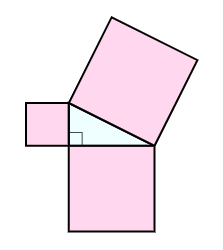
\includegraphics[width=0.4\textwidth]{../images/area13.png}
        \caption{}
        \label{fig:area13}
    \end{figure}

    \columnbreak

    \begin{parts}
        \part \textbf{¿Cuáles pueden ser las áreas de los cuadrados más pequeños?}
        \begin{checkboxes}
            \choice $15u^2$ y $20u^2$
            \CorrectChoice $6u^2$ y $30u^2$
            \choice $34u^2$ y $6u^2$
            \choice $10u^2$ y $16u^2$
            \CorrectChoice $26u^2$ y $10u^2$
            \CorrectChoice $24u^2$ y $12u^2$
            \choice $8u^2$ y $27u^2$
            \choice $6u^2$ y $6u^2$
        \end{checkboxes}
    \end{parts}\end{multicols}
